\documentclass[10pt]{extarticle}

% Lingua e matematica
\usepackage[english]{babel}
\usepackage{amsmath,amssymb,amsthm}

% Grafica e tabelle
\usepackage{graphicx}
\usepackage{subcaption}
\usepackage{float}
\usepackage{booktabs}
\usepackage{multirow}
\usepackage{siunitx}

% Codice (opzionale)
\usepackage{listings}
\usepackage{xcolor}
\definecolor{codegreen}{rgb}{0,0.6,0}
\definecolor{codegray}{rgb}{0.5,0.5,0.5}
\definecolor{codepurple}{rgb}{0.58,0,0.82}
\definecolor{backcolour}{rgb}{0.98,0.98,0.98}
\lstdefinestyle{mystyle}{
  backgroundcolor=\color{backcolour},
  commentstyle=\color{codegreen},
  keywordstyle=\color{magenta},
  numberstyle=\tiny\color{codegray},
  stringstyle=\color{codepurple},
  basicstyle=\ttfamily\footnotesize,
  breaklines=true, keepspaces=true, numbers=none, tabsize=2
}
\lstset{style=mystyle}

% Margini
\usepackage[margin=0.6in]{geometry}
\usepackage{ragged2e}
\usepackage{enumitem}
%\usepackage[utf8]{inputenc} % per caratteri UTF-8 nei .tex e nel .bib
\usepackage[backend=biber,style=ieee,sorting=none,maxbibnames=99]{biblatex}
\ExecuteBibliographyOptions{doi=true,url=true,isbn=false}
\addbibresource{references.bib}
\usepackage{csquotes}       % consigliato da biblatex (evita warning e parse strani)



% Bibliografia (biblatex + biber)
\usepackage[backend=biber,style=ieee]{biblatex}
\addbibresource{references.bib}

% TOC: includi anche \paragraph e numerali
\setcounter{secnumdepth}{2}
\setcounter{tocdepth}{2}

% Hyperref (sempre *dopo* gli altri pacchetti)
\usepackage[colorlinks=true,linkcolor=blue,citecolor=teal,urlcolor=magenta]{hyperref}


\begin{document}

% Custom header without a separate titlepage
\noindent
\begin{minipage}{0.3\textwidth}
    
\includegraphics[width=1.3\linewidth]{Figures/polito_logo_2021_blu.jpg}
\end{minipage}
\hfill
\begin{minipage}{0.68\textwidth}
    \raggedleft
    {\LARGE \textbf{Politecnico di Torino}}\\[0.2cm]
    {\large Master's Degree in Mathematical Engineering}\\[0.7cm]
    {\large \textbf{Material for Thesis}}\\[0.2cm]
    {\large a-- Exploratory Data Visualization of DNA Methylation \\in GSE69914}\\[0.7cm]
    \begin{tabular}{rl}
        Elisabetta Roviera & \texttt{s328422} \\
    \end{tabular}
\end{minipage}

\vspace{1cm}
\hrule
\vspace{0.5cm}

\tableofcontents

\vspace{0.5cm}
\hrule
\vspace{1cm}


% Main content begins here, on the same page
\justifying

\begin{abstract}
This report summarizes the exploratory visual analysis performed on the breast cancer methylation dataset GSE69914 \cite{ref6}. I first assess global distributions and quality, then quantify methylation outlier burden, contrast Tumor vs.\ Normal at the CpG level, and finally embed samples via dimensionality reduction. The goal is to establish a clear visual baseline before preprocessing the data. 

All supporting materials are available in the project repository: the full repo \href{https://github.com/elisabettaroviera/THESIS}{THESIS}, the curated medical/biological papers with summaries \href{https://github.com/elisabettaroviera/THESIS/tree/main/02%20-%20Paper/01%20-%20Medical%20and%20Biological%20information}{(Medical and Biological information)}, the data visualization papers and summaries \href{https://github.com/elisabettaroviera/THESIS/tree/main/02%20-%20Paper/03%20-%20Data%20EXPLORATION%20\%26%20VISUALIZATION}{(Data Exploration \& Visualization)}, and the complete notebook with all code that this document summarizes \href{https://github.com/elisabettaroviera/THESIS/blob/main/01%20-%20Notebook/01-data-exploration.ipynb}{(01-data-exploration.ipynb)}.
 
\end{abstract}

% ===================== 1. INTRO =====================
\section{Introduction}

Breast cancer represents one of the most extensively studied models of tumorigenesis and remains a leading cause of cancer-related mortality worldwide. 
Beyond genetic mutations, its initiation and progression are strongly influenced by epigenetic deregulation, particularly through alterations in DNA methylation patterns at cytosine–phosphate–guanine (CpG) sites \cite{ref4} \cite{ref8}. 
Such aberrant methylation contributes to transcriptional silencing of tumor-suppressor genes, genomic instability, and the establishment of pre-neoplastic “field defects” that precede visible malignancy \cite{ref12}.

The notebook, \textbf{01-data-exploration.ipynb}, constitutes the first computational step of my thesis project. 
Its goal is to perform an in-depth exploratory analysis and visualization of DNA methylation data from the \textbf{GSE69914} dataset \cite{ref6}, which profiles breast tissue samples from Normal, Tumor-adjacent, and Tumor contexts using the Illumina HumanMethylation450 BeadChip platform. 

The analyses presented here focus on establishing a clear and interpretable overview of the dataset’s global structure before applying any normalization or filtering. 
Specifically, the notebook explores:
\begin{itemize}[label=-]
    \item Global methylation distributions and sample-level variability;
    \item Methylation outlier burden and its progression across tissue groups;
    \item Group-level contrasts between Tumor and Normal samples at the CpG level; 
    \item Low-dimensional embeddings (t-SNE) capturing the overall organization of the methylome.
\end{itemize}

This exploratory phase provides the visual and quantitative foundation required for subsequent steps—namely, data preprocessing. 



% ===================== 2. DATASET =====================
\section{Dataset}
The \textbf{GSE69914} dataset \cite{ref6} provides DNA methylation profiles from \textbf{407 breast tissue samples} obtained using the \textbf{Illumina Infinium HumanMethylation450 BeadChip}, covering approximately \textbf{485,512 CpG sites}. It includes \textbf{56 normal tissues}, \textbf{49 adjacent tissues}, \textbf{302 tumors}, and a small subset of \textbf{BRCA1-related samples} (8 normal carriers and 3 tumors). After transposition, each row corresponds to a sample and each column to a CpG probe, with $\beta$-values in $[0,1]$ representing methylation levels. The array distinguishes CpG (\texttt{cg}) and non-CpG (\texttt{ch}) contexts \cite{ref9}. This dataset is an established reference for studying breast cancer epigenetics, and exhibits complete data coverage with no missing values, confirming its suitability for visualization and subsequent normalization.



% ===================== 3. VISUALIZATION =====================

\section{Visualization Pipeline and Key Findings}

The exploratory analysis of \textit{GSE69914} was designed as a stepwise visual pipeline, moving from global quality assessment to group comparison and, finally, to low-dimensional structure. The main results are summarized in Fig.~\ref{fig:vispanel}.

\subsection{Global methylation patterns and data quality}
I first examined the distribution of $\beta$-values (fractional DNA methylation in $[0,1]$) across individual samples.  
The per-sample density curves (Fig.~\ref{fig:vispanel1a}) show the characteristic \textbf{bimodal profile} of Illumina 450k arrays, with one peak near unmethylated CpGs ($\beta \approx 0$) and one near fully methylated CpGs ($\beta \approx 1$).  
This behaviour reflects the biology of CpG regulation, where many loci are either transcriptionally active (hypomethylated) or repressed (hypermethylated), rather than occupying stable intermediate states \cite{ref8,ref11}.  
When these distributions are stratified by group (Normal, Tumor-adjacent, Tumor; Fig.~\ref{fig:vispanel1b}), I observe that Tumor samples show a flatter high-$\beta$ peak and a broader tail, consistent with emerging \textbf{global hypomethylation} and higher heterogeneity.  
Tumor-adjacent samples tend to fall in between Normal and Tumor, suggesting early epigenetic drift in histologically non-tumor tissue \cite{ref12}.

\subsection{Group-wise summary at the sample level}
I then summarized each sample by its global methylation level and variability.  
The group-wise distributions of per-sample mean $\beta$ and dispersion (IQR) in Fig.~\ref{fig:vispanel1c} show two key trends:  
(i) \textbf{Tumor samples have slightly lower global methylation} than Normal, consistent with genome-wide hypomethylation being a hallmark of cancer and associated with genomic instability \cite{ref8};  
(ii) \textbf{Tumor samples are more variable}, indicating increased epigenetic instability and stochastic deregulation \cite{ref13}.  
This agrees with the outlier-burden analysis performed in the notebook, where Tumor carries a substantially higher number of CpG outliers than either Normal or Tumor-adjacent, mirroring the “instability load” phenotype reported in ageing and cancer epigenomes \cite{ref13}.

\subsection{Low-dimensional organization of the methylome}
To test whether these differences appear at a global, genome-wide level, I embedded all samples in two dimensions using a PCA$\rightarrow$t-SNE pipeline (Fig.~\ref{fig:vispanel1d}).  
Briefly, methylation profiles (expressed as M-values) were first compressed with PCA to the top 50 components, then projected into 2D using t-SNE.  
PCA captures major axes of variance, while t-SNE preserves local neighborhood structure in the reduced space \cite{ref15,ref16}.  
The resulting map shows \textbf{clear separation between Normal and Tumor samples}, with Tumor-adjacent samples occupying an intermediate region rather than overlapping completely with either group.  
This pattern supports a \textbf{continuous epigenetic gradient} from Normal $\rightarrow$ Tumor-adjacent $\rightarrow$ Tumor, instead of an abrupt “all-or-nothing” transition \cite{ref12}.

% Set a consistent target height for all subfigures
\newlength{\panelheight}
% --- VALORE RIDOTTO PER FAR STARE TUTTO IN UNA PAGINA ---
\setlength{\panelheight}{0.24\textheight} 

\begin{figure}[H]
    \centering

    % -------- Row 1: 1a + 1b --------
    \begin{subfigure}[t]{0.48\textwidth}
        \centering
        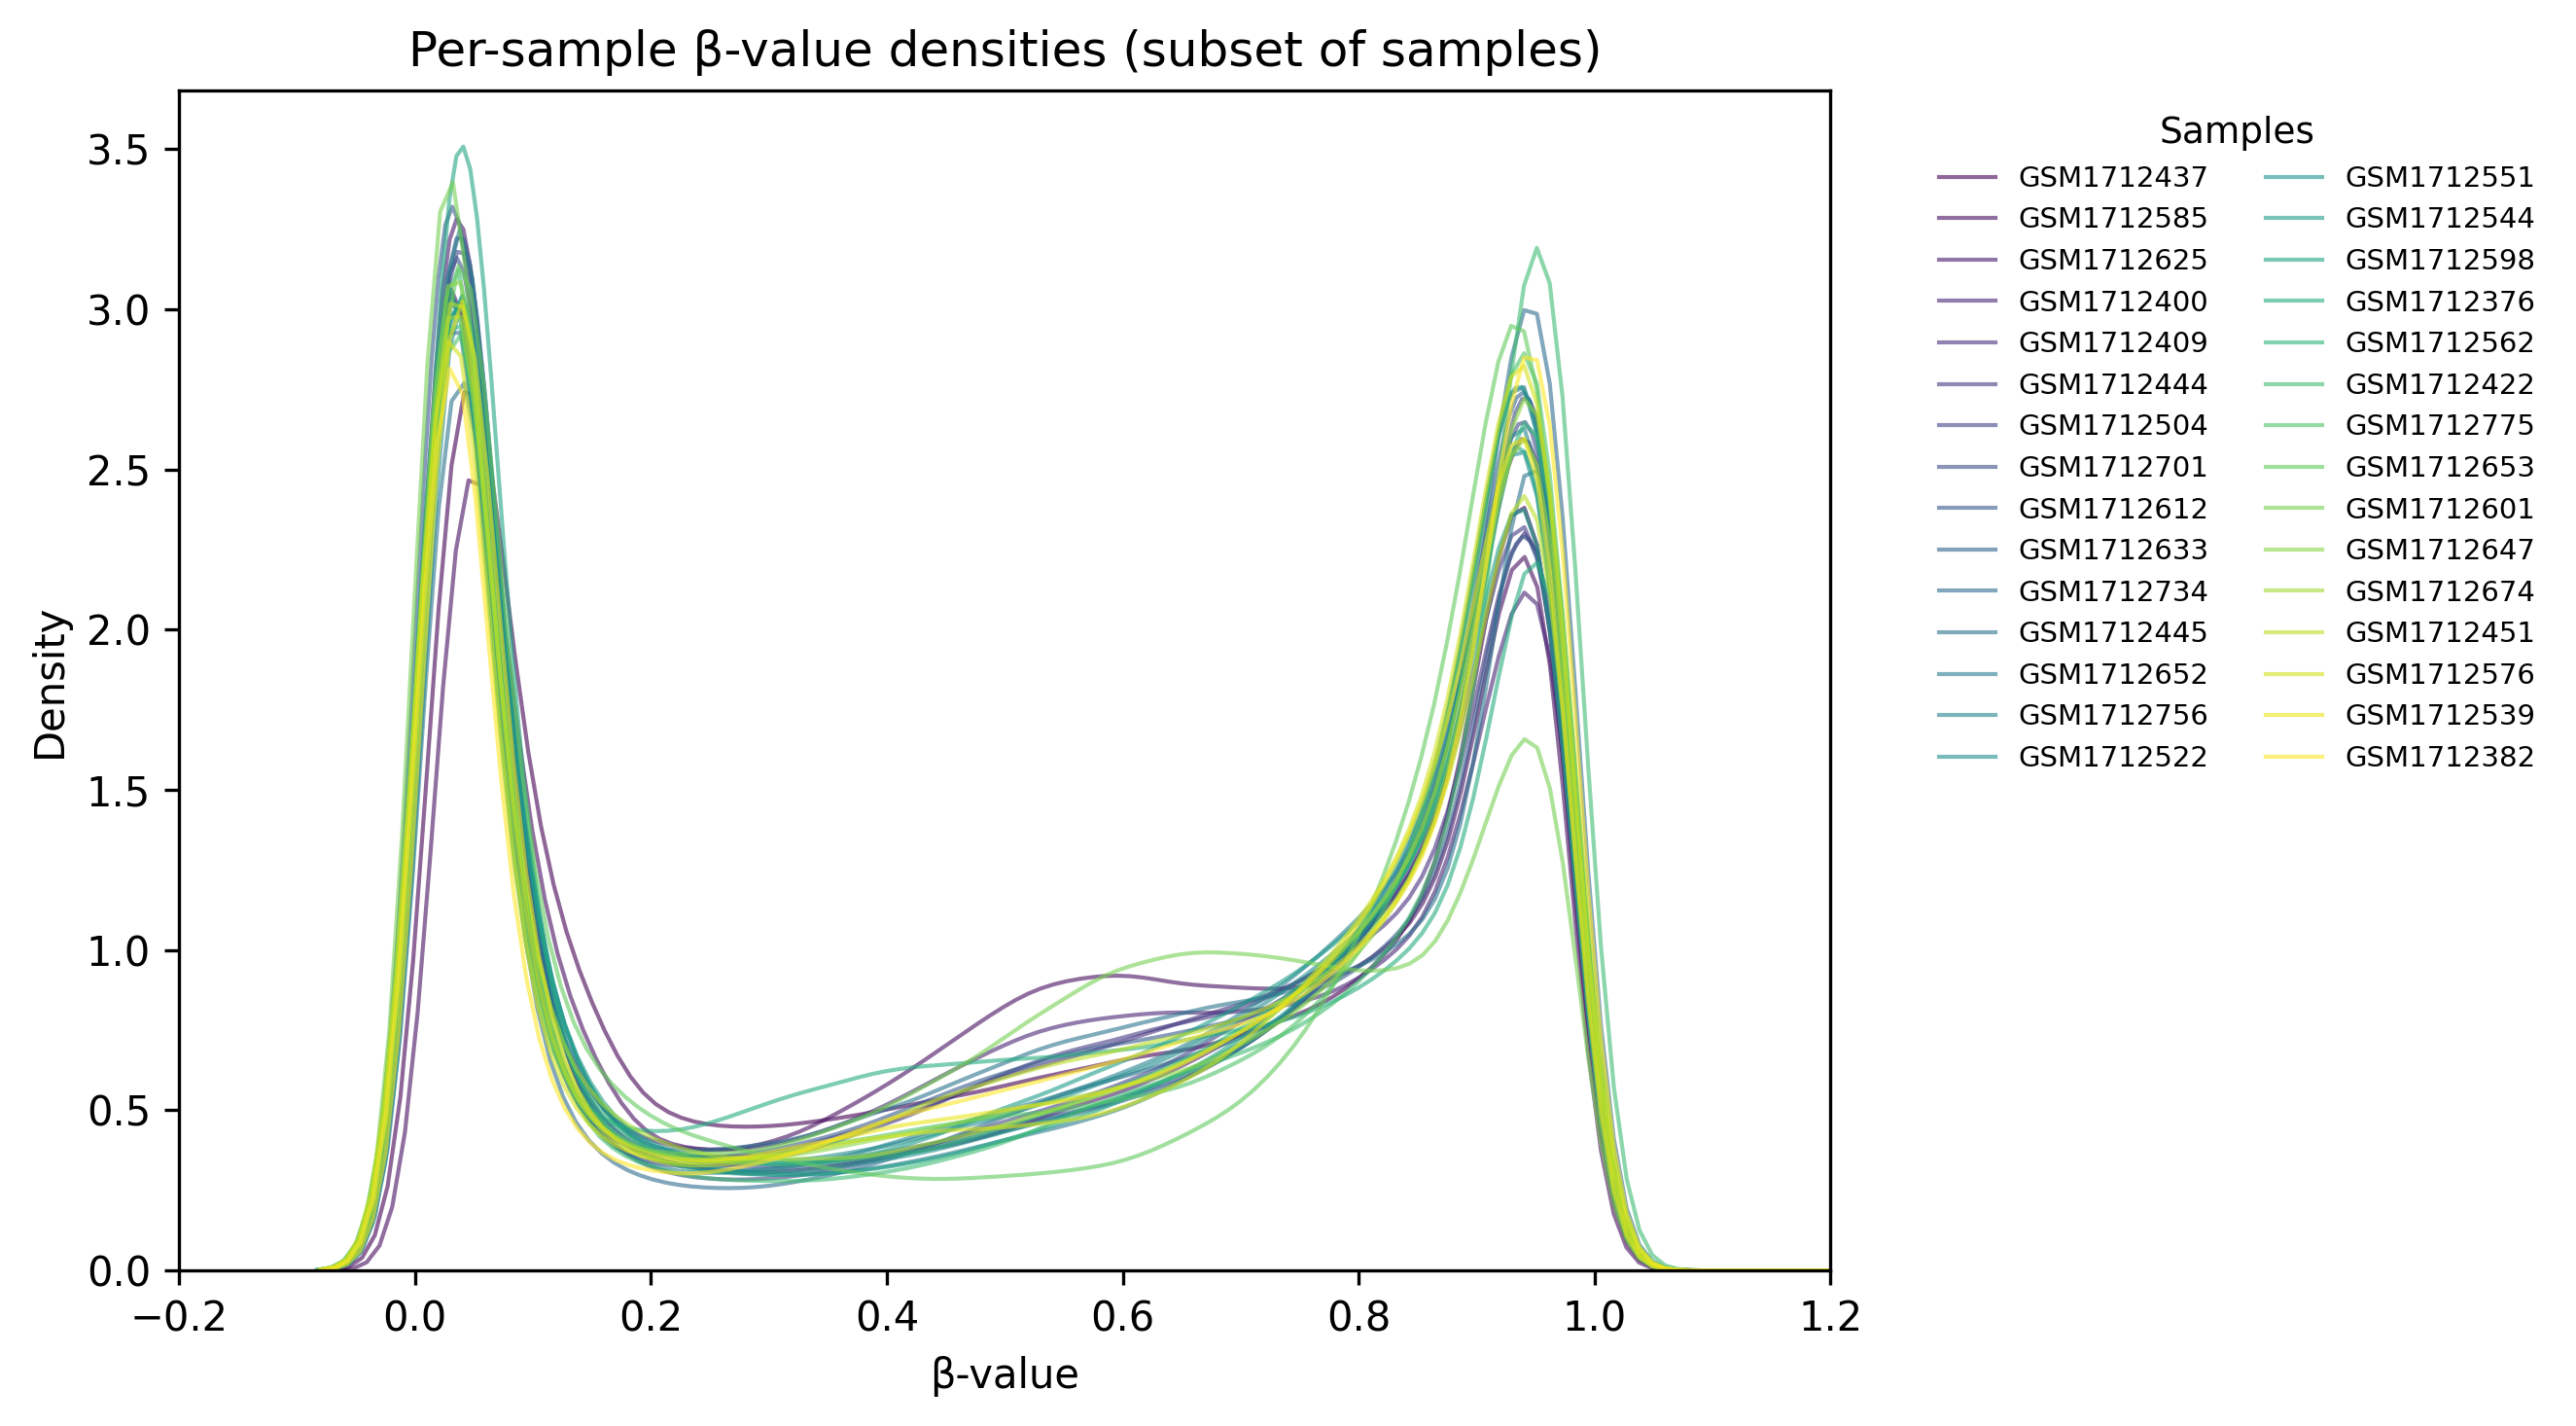
\includegraphics[height=\panelheight, width=\linewidth, keepaspectratio]{Figures/plot_1_1_global_beta_density_per_sample.png}
        \caption{Global $\beta$-value density per sample (bimodality check).}
        \label{fig:vispanel1a}
    \end{subfigure}
    \hfill
    \begin{subfigure}[t]{0.48\textwidth}
        \centering
        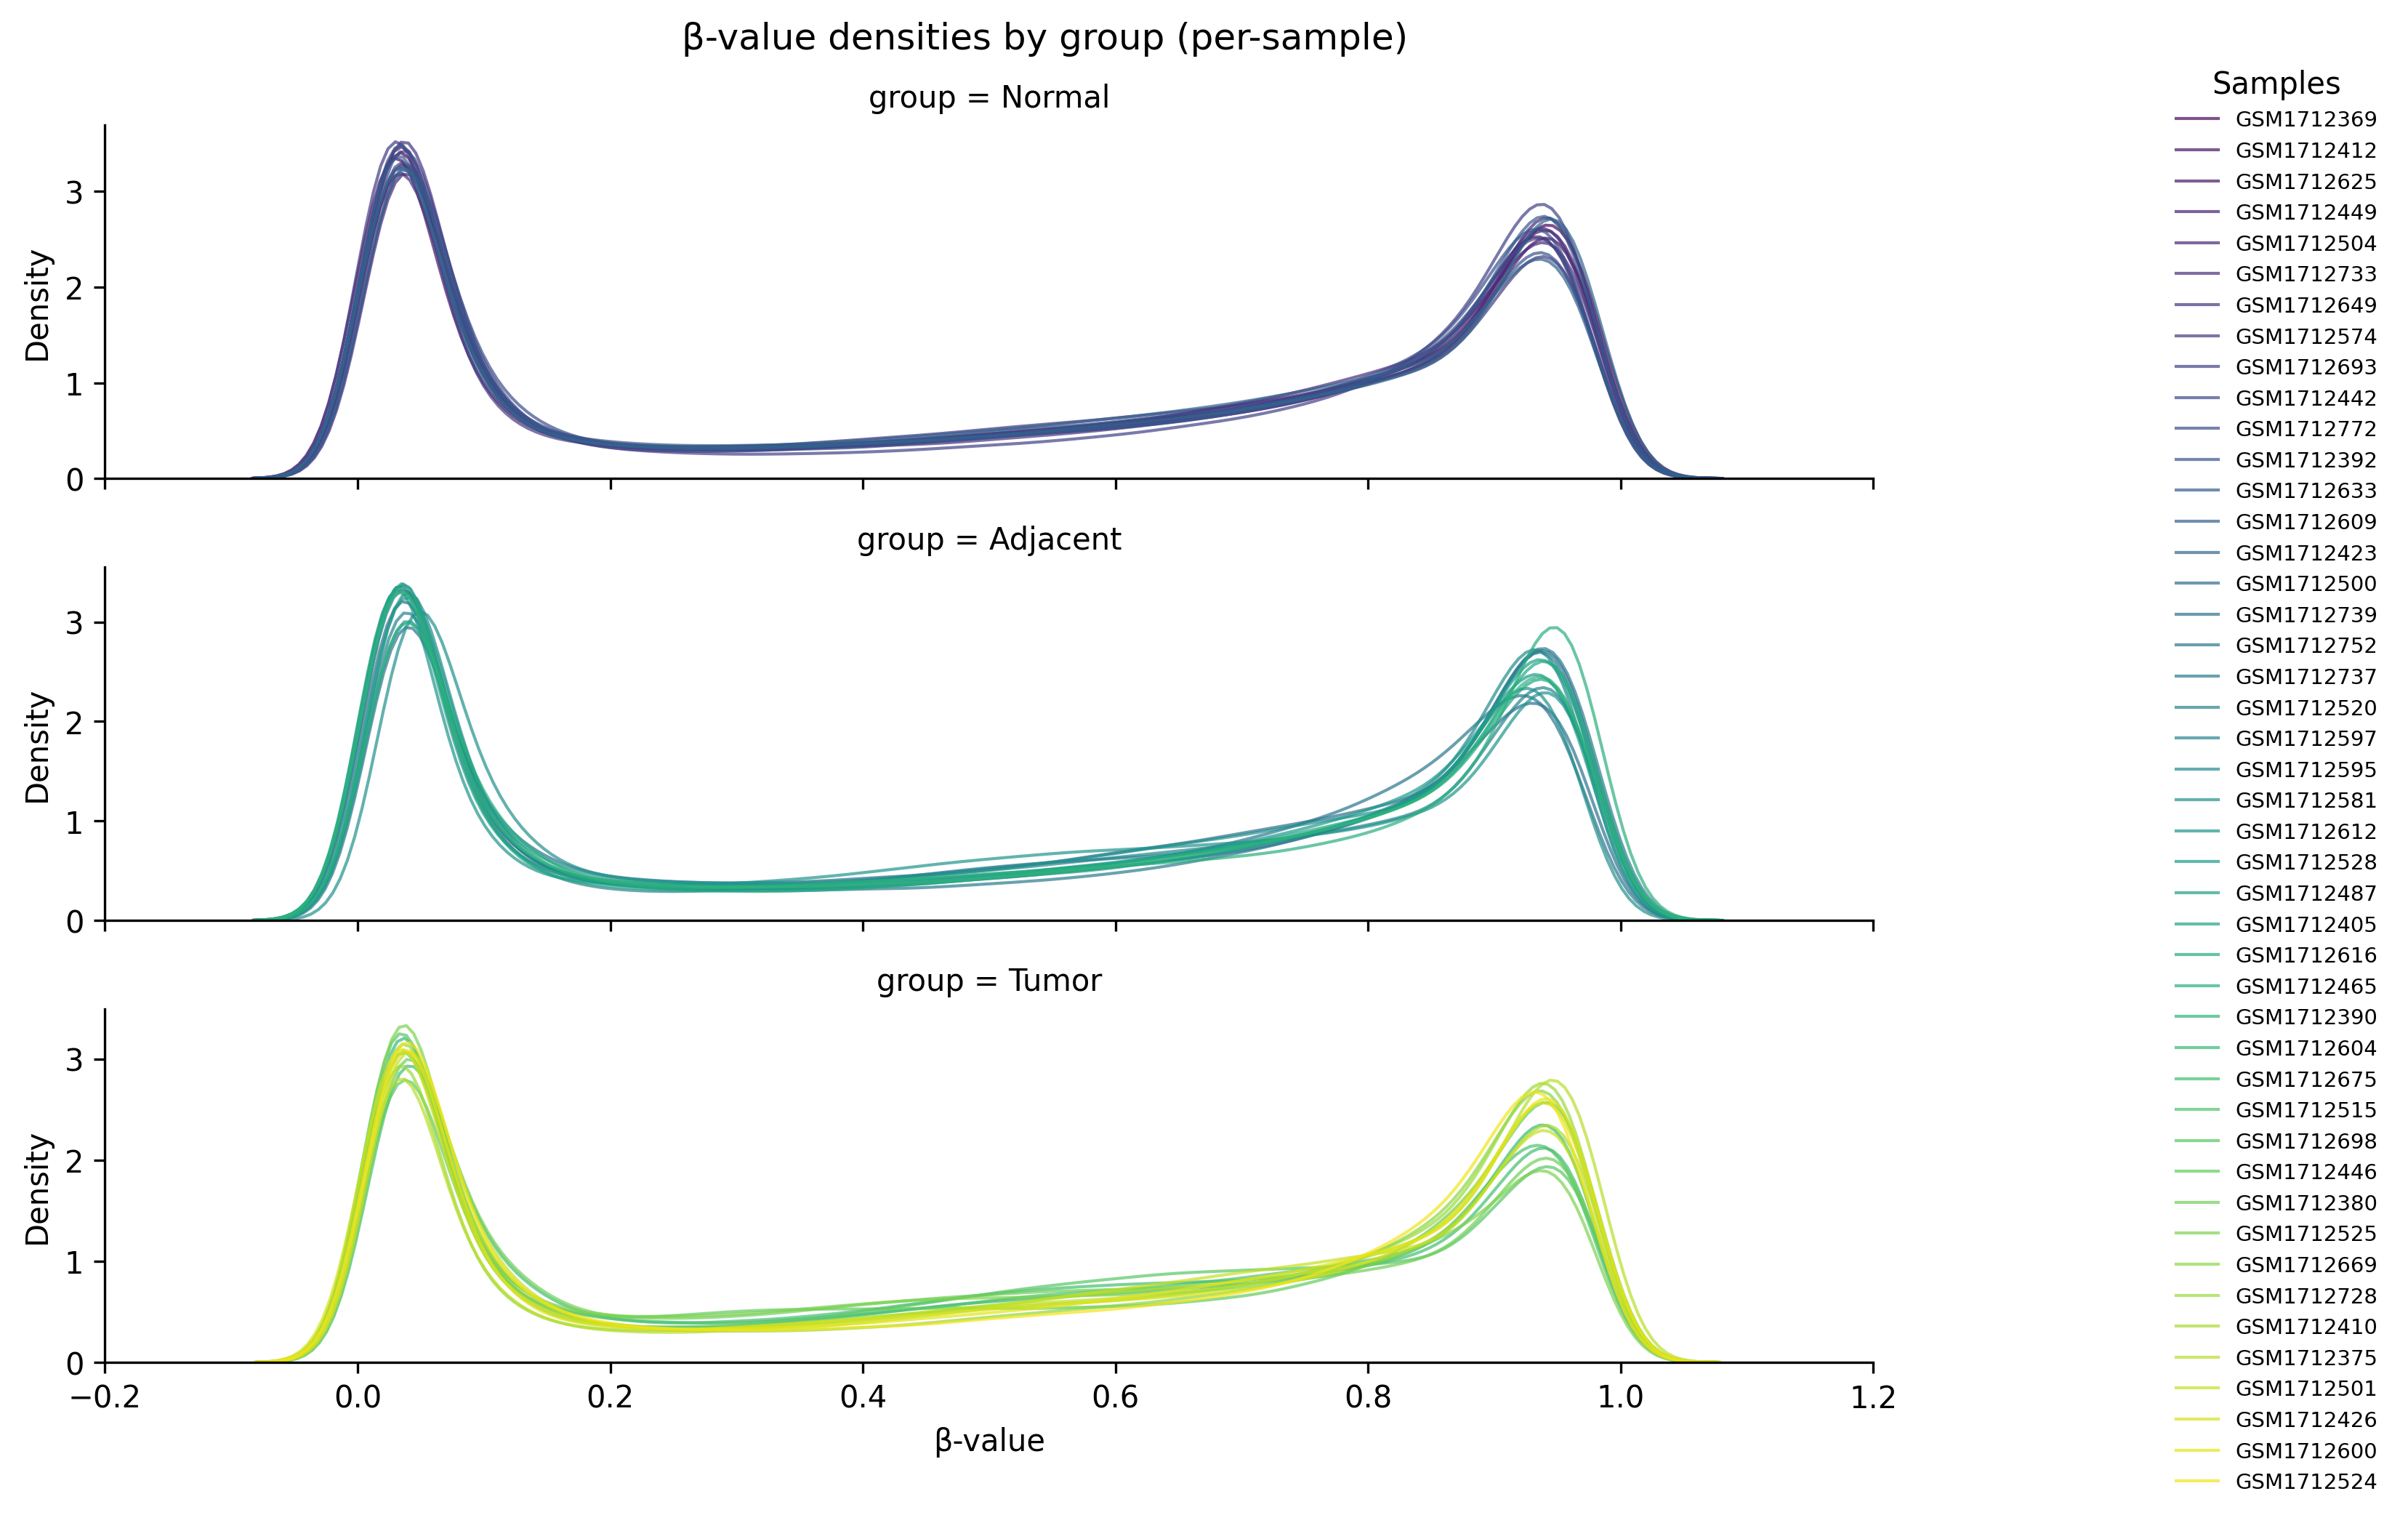
\includegraphics[height=\panelheight, width=\linewidth, keepaspectratio]{Figures/plot_1_2_Ridge_plot_by_group.png}
        \caption{Ridge plot by group.}
        \label{fig:vispanel1b}
    \end{subfigure}

    \vspace{1em}

    % -------- Row 2: 1c + 1d --------
    \begin{subfigure}[t]{0.48\textwidth}
        \centering
        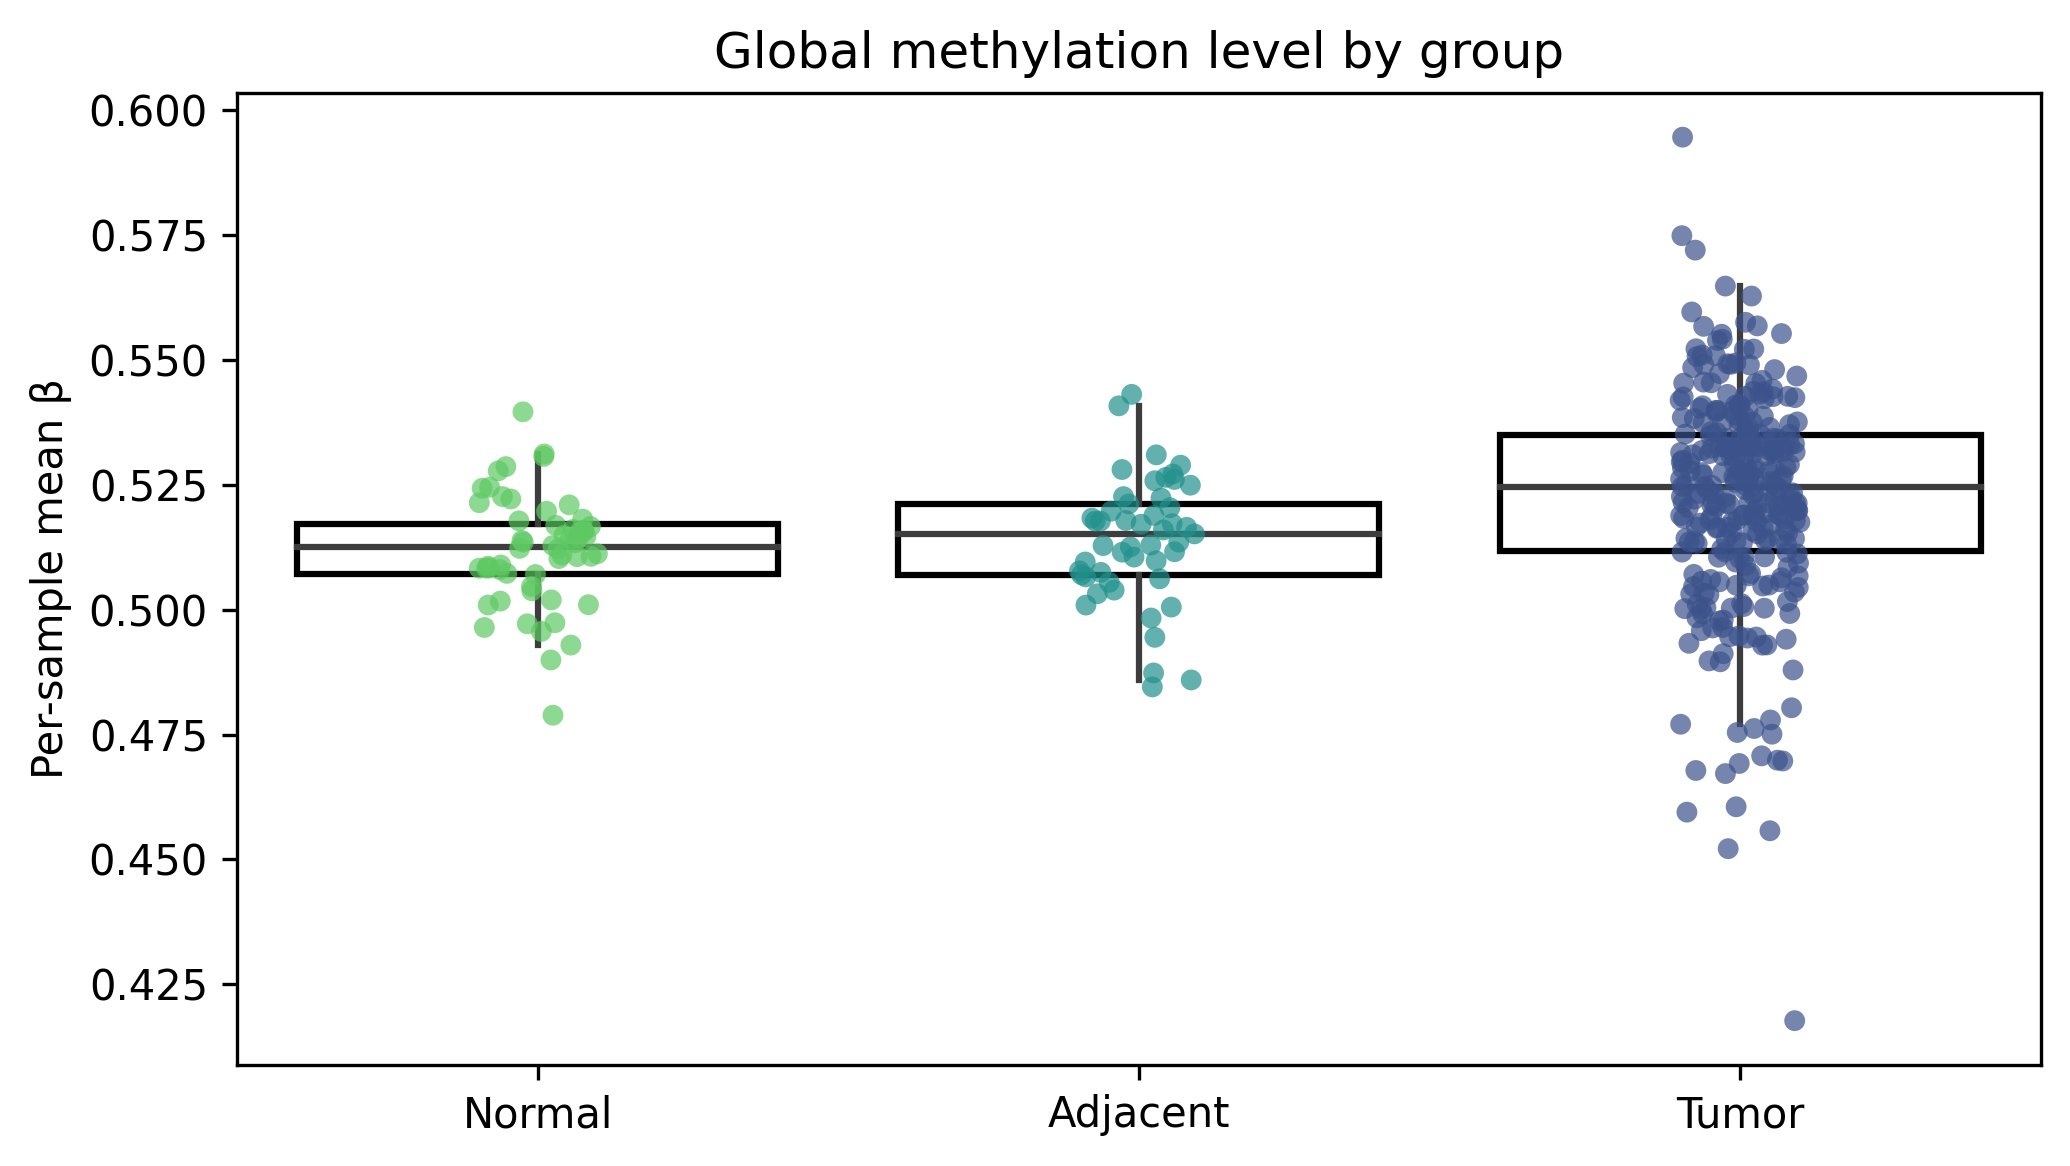
\includegraphics[height=\panelheight, width=\linewidth, keepaspectratio]{Figures/plot_1_4_Per_sample_summary_mean_β_and_IQR_β_by_group.png}
        \caption{Per-sample summary: mean $\beta$ and IQR $\beta$ by group.}
        \label{fig:vispanel1c}
    \end{subfigure}
    \hfill
    \begin{subfigure}[t]{0.48\textwidth}
        \centering
        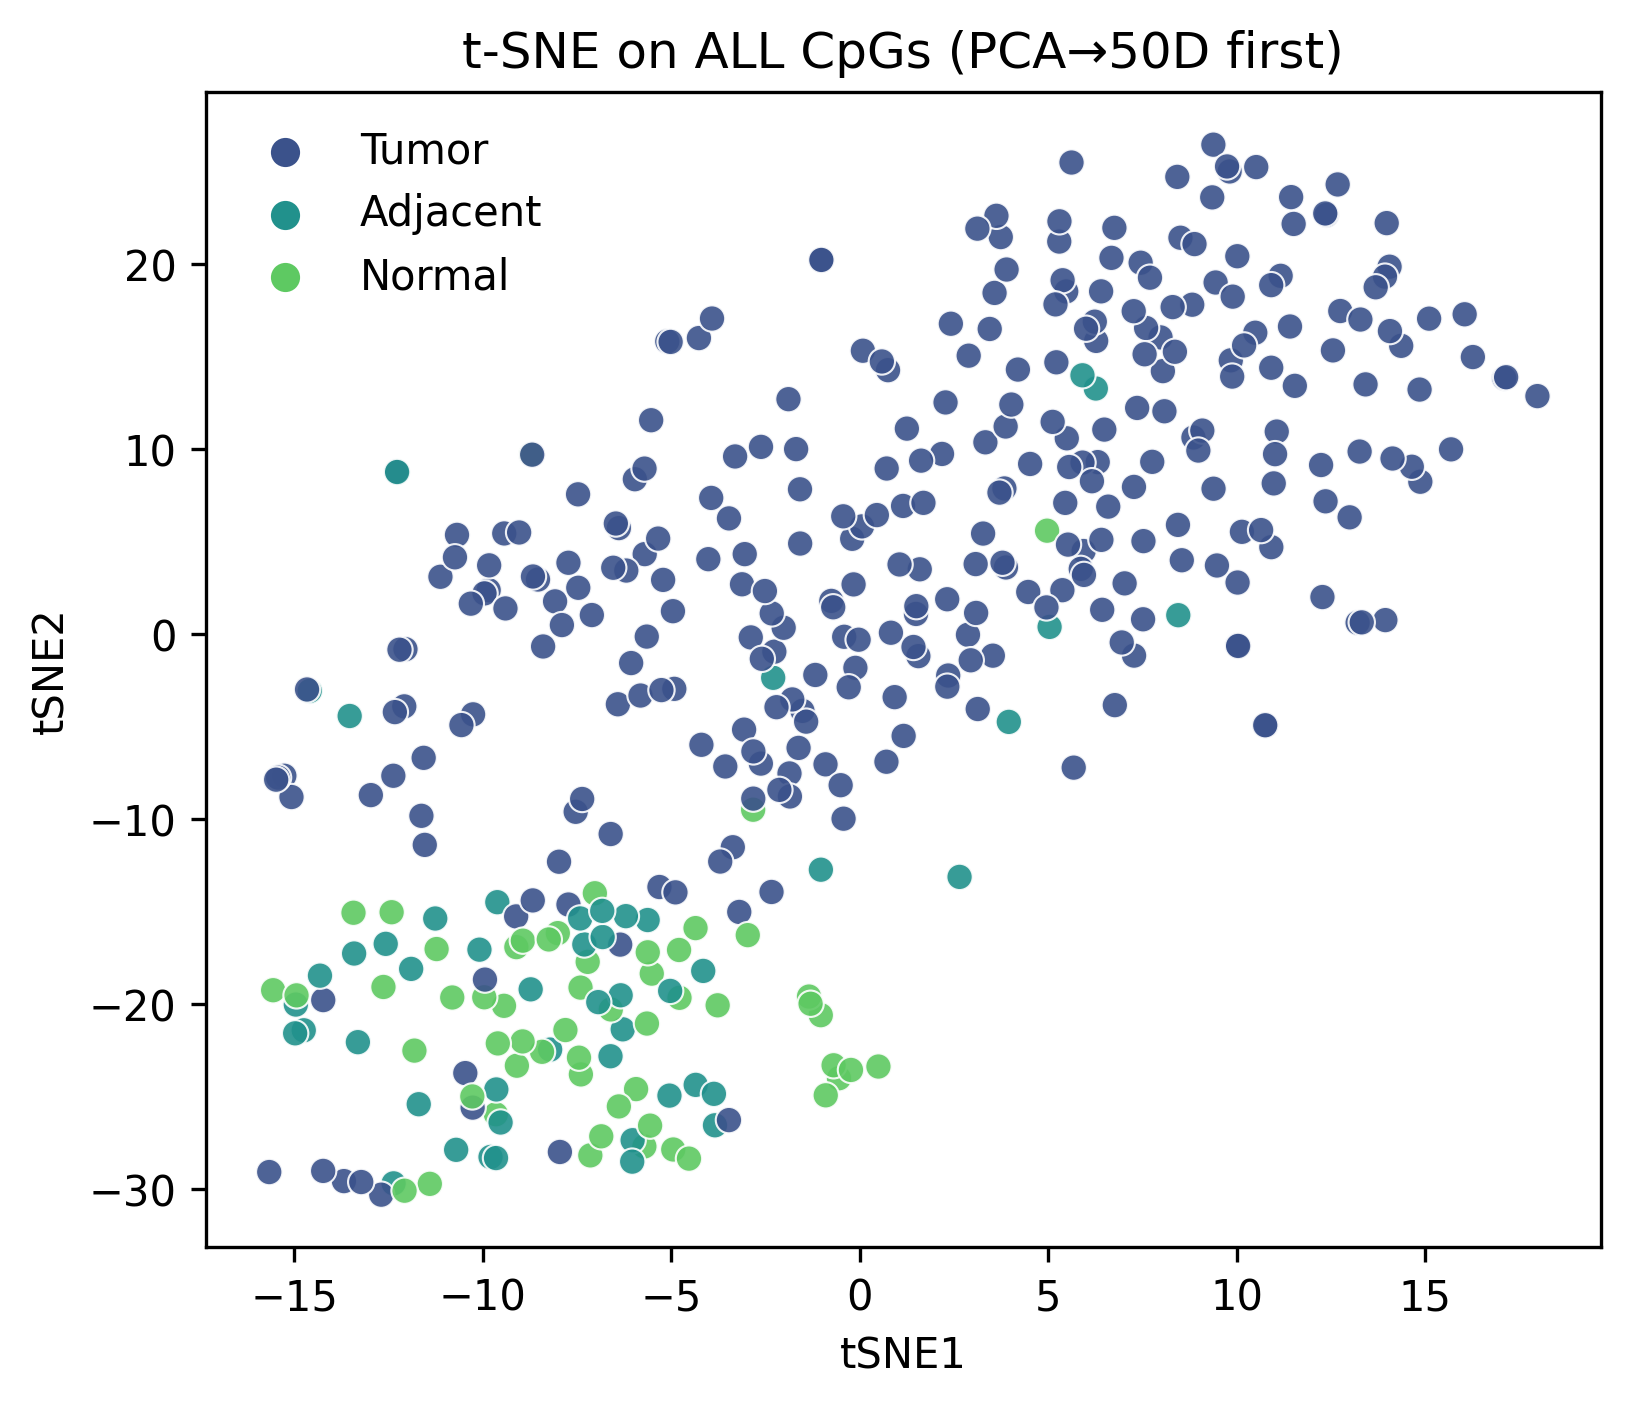
\includegraphics[height=\panelheight, width=\linewidth, keepaspectratio]{Figures/plot_4_1_t_SNE_using_ALL_CpGs_PCA_t_SNE.png}
        \caption{t-SNE using ALL $\sim$480k CpGs.}
        \label{fig:vispanel1d}
    \end{subfigure}

    \vspace{1em}

    % -------- Row 3: 1e full width --------
    \begin{subfigure}[t]{0.98\textwidth}
        \centering
        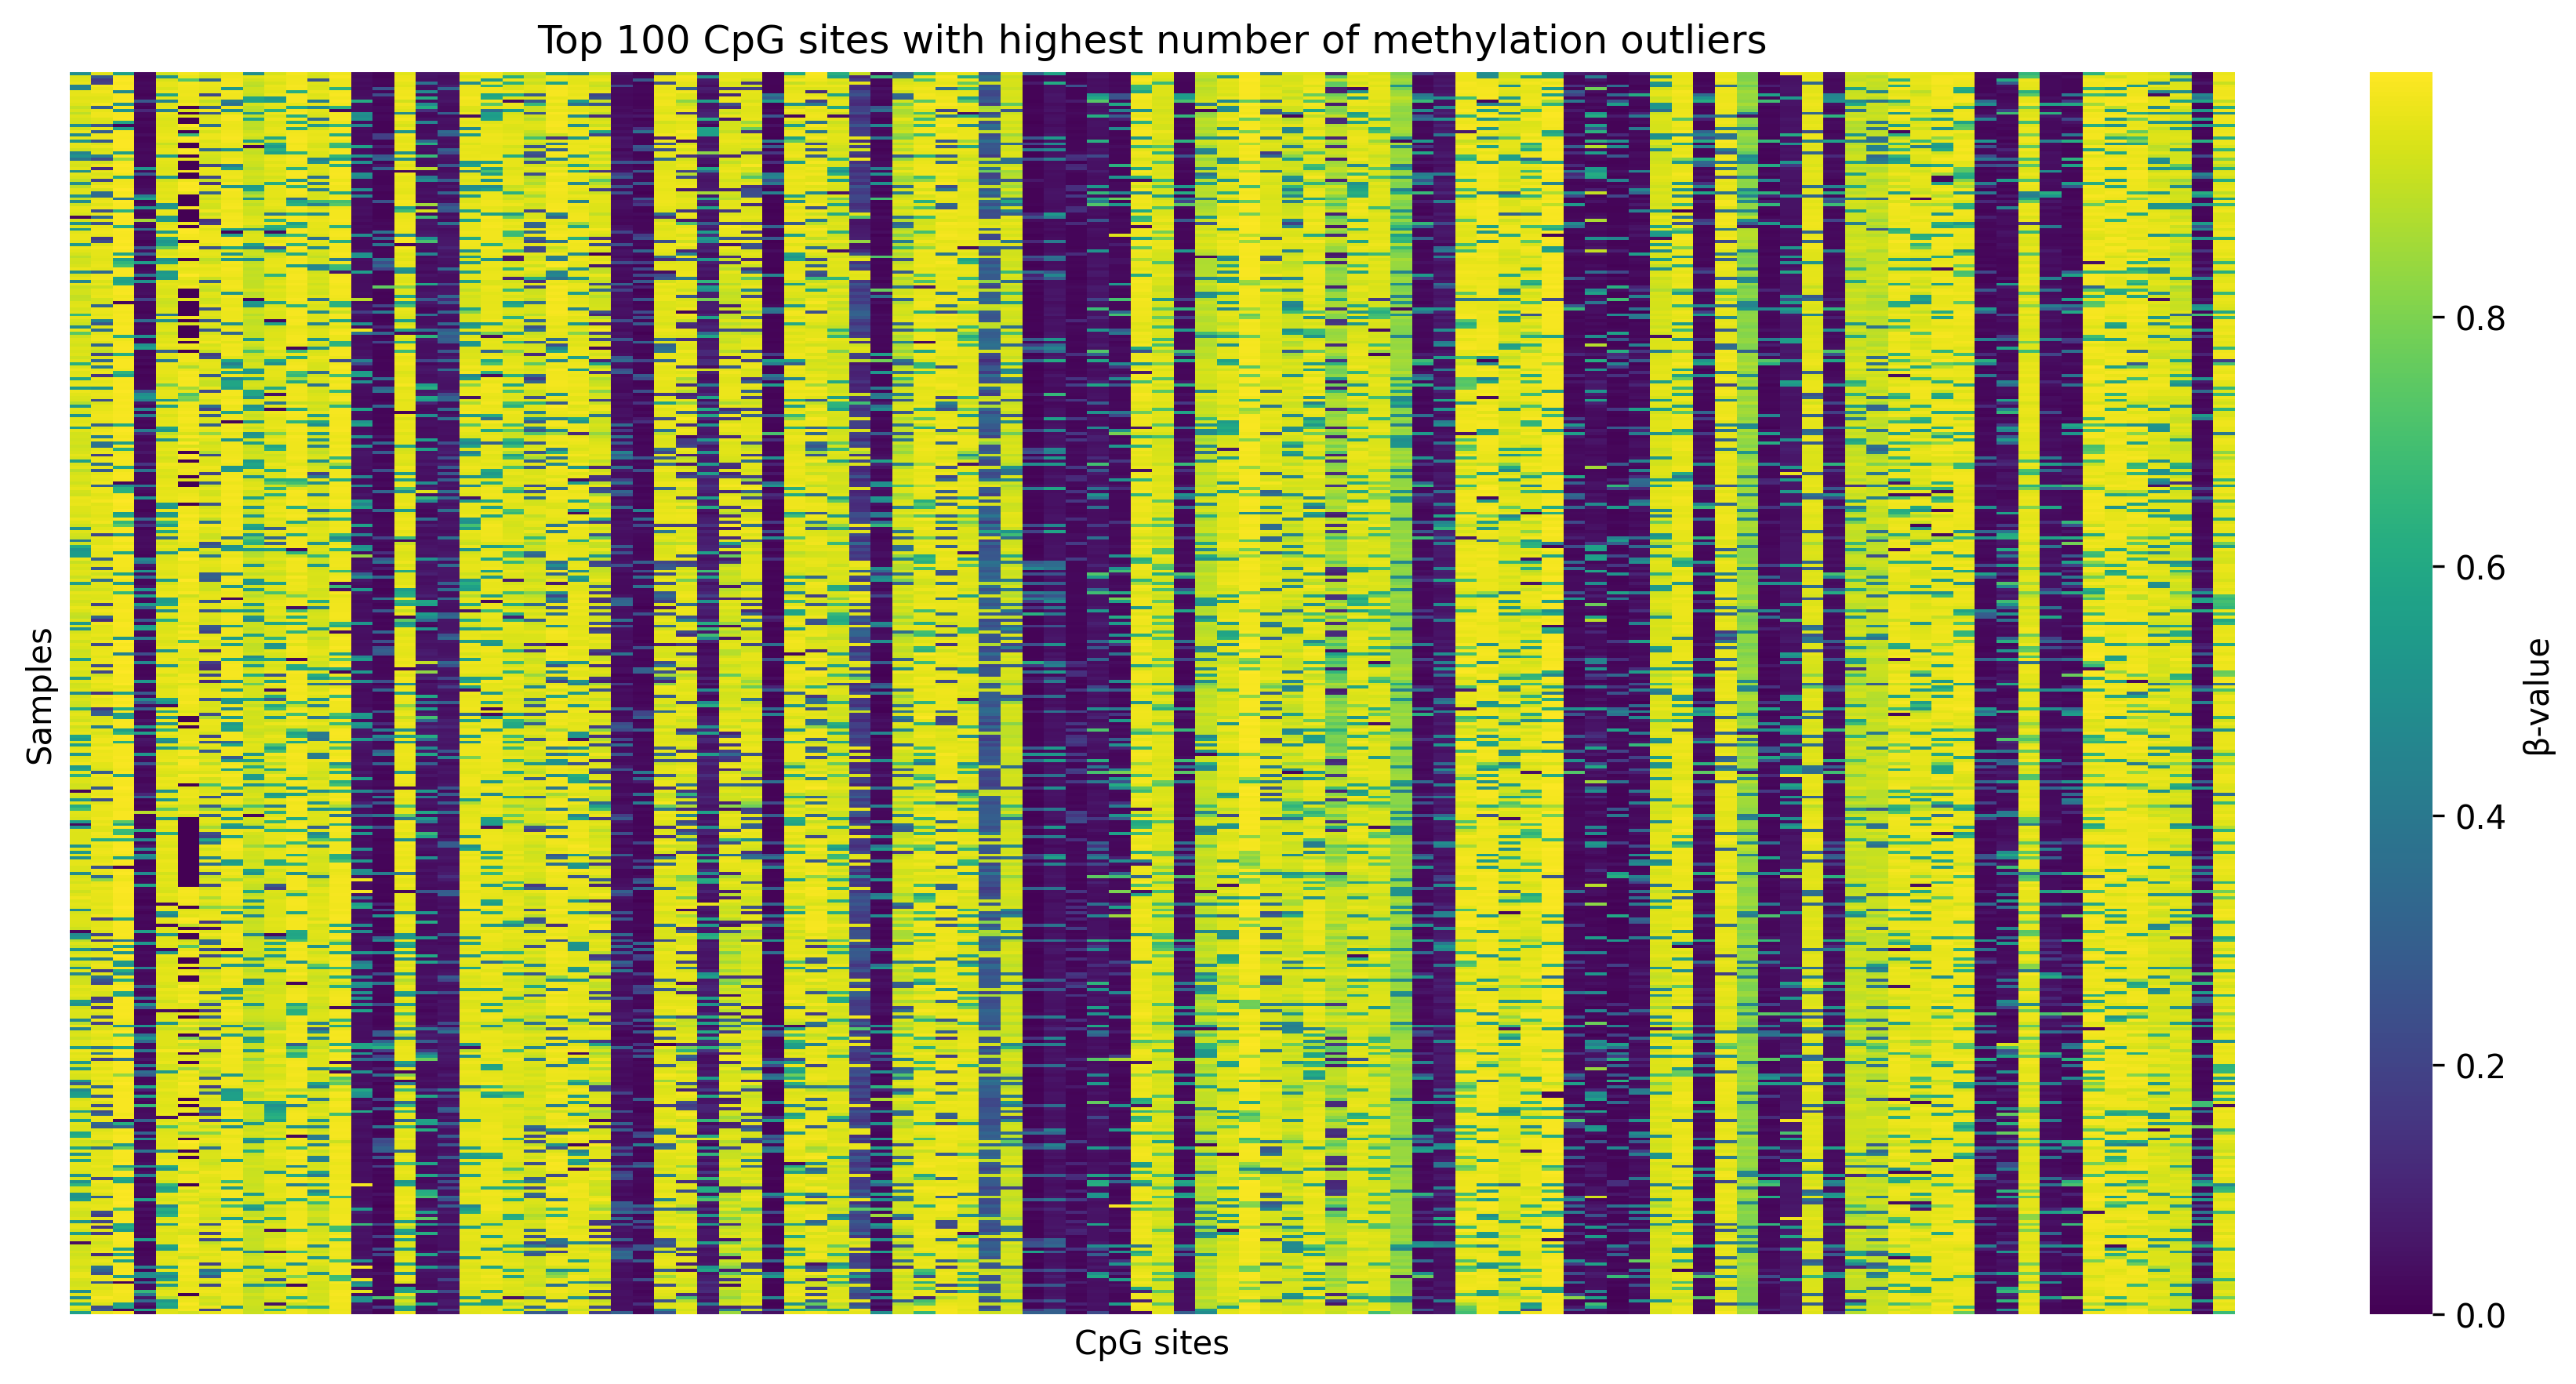
\includegraphics[height=\panelheight, width=0.98\linewidth, keepaspectratio]{Figures/plot_2_2_Heatmap_of_top_100_CpG_sites_with_the_highest_number_of_outliers.png}
        \caption{Heatmap of top 100 CpG outliers.}
        \label{fig:vispanel1e}
    \end{subfigure}

    \caption{
    Summary of the exploratory visual analysis of DNA methylation in \textit{GSE69914}.
    Panels~\ref{fig:vispanel1a}--\ref{fig:vispanel1b} show the expected bimodal distribution of $\beta$-values across samples, with systematic differences between Normal, Tumor-adjacent, and Tumor tissues.
    Panels~\ref{fig:vispanel1c}--\ref{fig:vispanel1d} highlight that Tumor samples display lower average methylation and markedly higher variability, and that a PCA$\rightarrow$t-SNE projection separates Normal and Tumor while placing Tumor-adjacent samples in between, suggesting a progressive epigenetic continuum rather than a binary switch \cite{ref12,ref13,ref15,ref16}.
    Panel~\ref{fig:vispanel1e} shows that recurrent CpG outliers arise in both directions (focal hypermethylation and focal hypomethylation), consistent with the known coexistence of promoter silencing and global/segmental demethylation in cancer \cite{ref8,ref11}.}
    \label{fig:vispanel}
\end{figure}

\subsection{Locus-level instability and recurrent CpG outliers}
Finally, I investigated which individual CpG sites show the most extreme deviations.  
The heatmap in Fig.~\ref{fig:vispanel1e} displays the top 100 CpG loci with the highest number of outlier events across samples.  
Two observations emerge:  
(i) epigenetic disruption is \textbf{not uniform} --- instability occurs at specific CpG sites and in specific samples, rather than as a smooth genome-wide shift;  
(ii) both directions are present --- I observe focal \textbf{hypermethylation} (very high $\beta$) and focal \textbf{hypomethylation} (very low $\beta$).  
In cancer biology, focal hypermethylation can silence tumor-suppressor regions, while focal hypomethylation can derepress oncogenic programs and weaken genomic stability \cite{ref8}.  
The coexistence of both extremes in the same tissue context reflects the classic “too much and too little methylation” behavior of tumor genomes \cite{ref8}.

% ===================== CONCLUSION =====================
\section{Conclusion}

These results are consistent with what I expect biologically and technically for HM450 data.  
Across multiple visualization strategies, results were consistent with known biological patterns:  
\begin{itemize}[label=-]
\item \textbf{Bimodal $\beta$-value distributions} typical of Illumina HM450 data;  
\item \textbf{Systematic group shifts}, with Tumor samples exhibiting lower global methylation and greater variability than Normal;  
\item \textbf{Intermediate profiles} for Tumor-adjacent tissues, suggesting early epigenetic drift rather than abrupt transitions \cite{ref12,ref13}.  
\end{itemize}

At the CpG level, heatmaps and boxplots highlighted \textbf{recurrently variable loci} where both focal hypermethylation and hypomethylation coexist—processes known to silence tumor suppressors and activate oncogenic pathways \cite{ref8}.  
Dimensionality-reduction results (PCA~$\rightarrow$~t-SNE) further supported a \textbf{continuous epigenetic gradient} from Normal to Tumor, confirming structured rather than random methylation differences.

\vspace{0.3cm}

\noindent Overall, these findings validate the dataset’s quality and provide a strong rationale for the upcoming \textit{data pre-processing} phase.  





\printbibliography
\end{document}
